% =====================================================================
%  Orientation Reconstruction of a Tennis Stroke from a Dampener-Mounted
%  6-Axis IMU, with Two-View Video Validation and Gaussian-Process
%  Drift Correction -- scientific report (pdfLaTeX, single file).
%
%  Figures are loaded from img/ if present (stroke_frames.png,
%  contact_sensor_only.png, contact_gp.png, gp_plot.png); otherwise a
%  labelled placeholder is drawn, so the file compiles on its own.
% =====================================================================
\documentclass[11pt,a4paper]{article}
\usepackage[T1]{fontenc}
\usepackage[utf8]{inputenc}
\usepackage{lmodern}
\usepackage[margin=2.5cm]{geometry}
\usepackage{amsmath,amssymb,bm}
\usepackage{booktabs,array}
\usepackage{siunitx}
\usepackage{graphicx}
\usepackage{xcolor}
\usepackage[font=small,labelfont=bf]{caption}
\usepackage{float}
\usepackage{enumitem}
\usepackage{tikz}
\usetikzlibrary{arrows.meta,positioning,calc}
\usepackage[hidelinks]{hyperref}

\sisetup{detect-all}
\setlength{\parskip}{0.35em}

% ---------- notation ----------
\newcommand{\q}{\bm{q}}
\newcommand{\qv}{\bm{v}}
\newcommand{\w}{\bm{\omega}}
\newcommand{\Rm}{\mathbf{R}}
\newcommand{\ve}[1]{\bm{#1}}
\newcommand{\qmul}{\otimes}
\newcommand{\dg}{^{\circ}}
\newcommand{\Exp}{\operatorname{Exp}}
\newcommand{\Log}{\operatorname{Log}}
\newcommand{\norm}[1]{\left\lVert #1 \right\rVert}

\newcommand{\maybefig}[3][\linewidth]{%
  \IfFileExists{img/#2}{\includegraphics[width=#1]{img/#2}}{%
    \fbox{\parbox[c][3cm][c]{0.9\linewidth}{\centering\small\color{gray}
      Figure file \texttt{img/#2} not provided.\\ #3}}}}

\title{\textbf{Orientation Reconstruction of a Tennis Stroke from a\\
Dampener-Mounted Inertial Sensor, with Two-View Video Validation\\
and Gaussian-Process Drift Correction}}
\author{[Author names]\\[0.3em]
\small [Affiliation]\\
\small [Contact e-mail]}
\date{October 2026}

\begin{document}
\maketitle

% ---------------------------------------------------------------------
\begin{abstract}
\noindent\textbf{Background.} Low-cost inertial sensors attached to sports equipment could replace
camera-based motion capture, but a single short, saturated recording without a static period is a
difficult case for orientation estimation.
\textbf{Methods.} We reconstruct the three-dimensional orientation of a tennis racket through one
forehand from a 6-axis inertial measurement unit (IMU) embedded in a string dampener (400 samples
at \SI{416}{Hz}, accelerometer saturated at \SI{16}{g} before impact). Orientation is computed by
strapdown integration of the angular rate with exact exponential quaternion updates. An independent
reference is obtained from two uncalibrated videos by a two-camera bundle adjustment that uses the
racket as the calibration object. Saturated acceleration is reconstructed from a centripetal model,
and a Gaussian process (GP) models the residual orientation error between sensor and video.
\textbf{Results.} The integrator has a maximum error of $0.027\dg$ on a synthetic
$\approx500\dg/\mathrm{s}$ moving-axis rotation at the sensor rate. From the IMU alone we obtain a
peak angular rate of $1720\dg/\mathrm{s}$, an estimated racket-head speed at impact of
\SI{24.6}{m/s}, a reconstructed peak acceleration of approximately \SI{30}{g}, and a string
vibration aliased to \SI{164.5}{Hz} (most plausibly \SI{581}{Hz}). The sensor-only orientation
agrees with video within $2$--$11\dg$ in the early swing and diverges in the fast phase. GP drift
correction reduces the leave-one-out angular error against video from a mean of $88.4\dg$ to
$12.4\dg$ (median $8.3\dg$).
\textbf{Conclusions.} A dampener-sized IMU recovers the stroke's orientation and key kinematic
parameters; residual sensor--video disagreement in the fastest phase points to inter-device time
synchronisation as the main open problem.
\end{abstract}

\noindent\textbf{Keywords:} inertial measurement unit; strapdown integration; quaternions; bundle
adjustment; Gaussian process regression; tennis; sports telemetry.

% =====================================================================
\section{Introduction}
% =====================================================================
Racket-mounted sensors are an inexpensive alternative to optical motion capture for stroke
analysis. A 6-axis IMU measures angular rate and specific force in its own frame; orientation
follows from integrating the angular rate, and position, in principle, from double integration of
acceleration once orientation and gravity are known. In practice the problem is shaped by three
constraints: the integration constant (the initial orientation) is unobservable from the gyroscope,
integration accumulates error (drift), and accelerometers of consumer devices saturate during fast
motion.

Attitude integration from angular rate is a classical topic in inertial navigation. The rotation
vector formulation of Bortz~\cite{bortz1971} and the algorithm-design analysis of
Savage~\cite{savage1998} describe high-order attitude updates and the coning error that arises when
the rotation axis moves within an update interval. Quaternion kinematics, including the exponential
and logarithm maps used here, are summarised by Sol\`a~\cite{sola2017}. Averaging of orientation
estimates on the unit-quaternion manifold follows Markley et al.~\cite{markley2007}.

For the video reference we rely on multi-view geometry~\cite{hartley2004} and bundle
adjustment~\cite{triggs2000}, the joint non-linear least-squares refinement of camera and structure
parameters. Camera calibration from a known planar object is classical~\cite{zhang2000}; planar
pose estimation with the IPPE method~\cite{collins2014} requires a homography, which is degenerate
for our point configuration (Section~\ref{sec:ba}). The residual sensor--video error is modelled by
Gaussian process regression~\cite{rasmussen2006}, implemented with scikit-learn~\cite{sklearn2011};
numerical optimisation uses SciPy~\cite{scipy2020}.

This report makes four contributions: (i) a verified orientation pipeline for a short, mid-swing,
saturated IMU record; (ii) a two-view reconstruction of the racket that needs no calibration target
other than the racket itself; (iii) sensor-only estimates of the stroke's kinematic parameters,
including a physical reconstruction of the saturated acceleration; and (iv) a quantitative,
leave-one-out comparison of sensor-only and GP-corrected orientation against video, together with
an explicit account of the hypotheses tested for the residual disagreement.

% =====================================================================
\section{Materials and methods}
% =====================================================================
\subsection{Data}\label{sec:data}
\paragraph{Inertial data.} The record contains $N=400$ samples of specific force
$(a_x,a_y,a_z)$ in units of $g$ and angular rate $(\omega_x,\omega_y,\omega_z)$ in degrees per
second, sampled at $f_s=\SI{416}{Hz}$ ($t_k=k/f_s$; duration \SI{0.962}{s}). Impact occurs at
sample 200, marked by a one-sample discontinuity in both sensors followed by string ringing. The
record begins mid-swing, so no static interval is available. The $x$ accelerometer channel is
saturated at \SI{15.96}{g} on samples 182--199; the peak angular rate, $1720.1\dg/\mathrm{s}$ at
sample 199, is below the gyroscope range. Table~\ref{tab:imu} summarises the record.

\begin{table}[H]\centering\small
\caption{Properties of the IMU record.}\label{tab:imu}
\begin{tabular}{@{}ll@{}}\toprule
Samples, rate, duration & 400, \SI{416}{Hz}, \SI{0.962}{s} \\
Impact sample & 200 \\
Peak $\norm{\w}$ & $1720.1\dg/\mathrm{s}$ (sample 199) \\
Peak $|\omega_x|,|\omega_y|,|\omega_z|$ & $1232$, $1286$, $1228\dg/\mathrm{s}$ \\
Accelerometer saturation & $a_x=\SI{15.96}{g}$, samples 182--199 \\
Gyroscope at samples 199, 200, 201 & $(791,-1276,840)$, $(793,-766,804)$, $(1134,116,521)\dg/\mathrm{s}$\\
Static interval & none \\\bottomrule
\end{tabular}
\end{table}

\paragraph{Sensor frame.} The sensor is mounted on the string bed near the throat. Its
right-handed axes are $x$ along the handle towards the butt, $y$ across the string face and $z$
normal to the string face (Fig.~\ref{fig:frame}). The $x$ axis is supported by the data: under
rotation about a pivot at distance $r$ in the $-x$ direction, the $x$ channel contains the
centripetal term
\begin{equation}
a_x \approx r\,\omega_\perp^2,\qquad \omega_\perp^2=\omega_y^2+\omega_z^2 ,
\label{eq:centripetal}
\end{equation}
and the observed correlation between $a_x$ and $\omega_\perp^2$ is $0.92$ before impact (samples
0--181) and $0.99$ after it (samples 231--399). The sign convention of positive rotation was not
specified and is determined in Section~\ref{sec:start}.

\begin{figure}[H]\centering
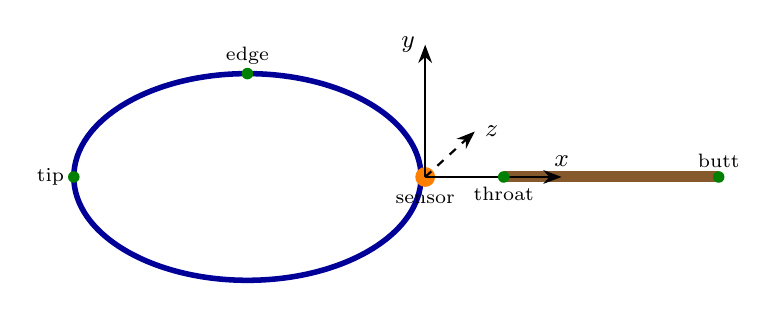
\begin{tikzpicture}[scale=1.05,>=Stealth]
  \draw[line width=4pt,brown!70!black] (0,0) -- (2.6,0);
  \draw[line width=2pt,blue!60!black] (-3.1,0) ellipse (2.1 and 1.25);
  \fill[orange] (-0.95,0) circle (0.12);
  \node[below=3pt,font=\scriptsize] at (-0.95,0) {sensor};
  \draw[->,thick] (-0.95,0) -- (0.7,0) node[above,font=\small]{$x$};
  \draw[->,thick] (-0.95,0) -- (-0.95,1.6) node[left,font=\small]{$y$};
  \draw[->,thick,dashed] (-0.95,0) -- (-0.35,0.55) node[right,font=\small]{$z$};
  \foreach \pt/\lab/\pos in {{(2.6,0)}/butt/above,{(0,0)}/throat/below,{(-5.2,0)}/tip/left,{(-3.1,1.25)}/edge/above}
     {\fill[green!50!black] \pt circle (0.07); \node[\pos,font=\scriptsize] at \pt {\lab};}
\end{tikzpicture}
\caption{Racket, sensor frame and the four anchor points annotated in the videos.}
\label{fig:frame}
\end{figure}

\paragraph{Video data.} Two videos (1280$\times$720 pixels, approximately 30 frames per second)
record the stroke from the front and from an oblique rear viewpoint. Impact is at front frame 131
and rear frame 172 (front frame $n$ corresponds to rear frame $n+41$). For the 29 frames within the
IMU window, the image positions of four racket points (butt, throat, tip and edge of the head) were
annotated manually in both views. Moment $i$ corresponds to the fractional IMU sample
$s_i=200+f_s\,t_i$, with $t_i$ the time from impact. Decoded presentation timestamps agree with
$t_i$ in both views. One annotation error was found and corrected: in front frame 118 the four
labels were cyclically permuted.

\subsection{Orientation representation}\label{sec:quat}
Orientations are unit quaternions $\q=(q_w,\qv)$ with the Hamilton product
\begin{equation}
\q_1\qmul\q_2=\bigl(w_1w_2-\qv_1\!\cdot\!\qv_2,\; w_1\qv_2+w_2\qv_1+\qv_1\times\qv_2\bigr),
\end{equation}
and $\q$ maps body-frame vectors to the world frame,
$(0,\ve u_{\mathrm w})=\q\qmul(0,\ve u_{\mathrm b})\qmul\q^{-1}$. The exponential map of a rotation
vector $\ve\phi=\theta\hat{\ve n}$ and its inverse are~\cite{sola2017}
\begin{equation}
\Exp(\ve\phi)=\Bigl(\cos\tfrac{\theta}{2},\,\frac{\sin(\theta/2)}{\theta}\,\ve\phi\Bigr),\qquad
\Log(\q)=\frac{2\,\operatorname{atan2}(\norm{\qv},q_w)}{\norm{\qv}}\,\qv\quad(q_w\ge0),
\label{eq:exp}
\end{equation}
with a series expansion for $\theta<10^{-8}$. The geodesic distance is
$d(\q_1,\q_2)=2\arccos|\q_1\cdot\q_2|$, and orientations at fractional sample indices are obtained
by spherical linear interpolation,
$\operatorname{slerp}(\q_1,\q_2,u)=\q_1\qmul\Exp\bigl(u\Log(\q_1^{-1}\qmul\q_2)\bigr)$.
Integrated series are kept sign-continuous ($\q_k\cdot\q_{k-1}>0$).

\subsection{Strapdown integration}\label{sec:gyro}
With bias $\ve b$ and sign convention $\sigma\in\{+1,-1\}$, the body rate is
$\w_k=\sigma\frac{\pi}{180}(\tilde{\w}_k-\ve b)$. The kinematic equation
$\dot{\q}=\tfrac12\q\qmul(0,\w)$ is integrated with the mean rate over each interval
$\Delta t=1/f_s$ and an exact exponential step:
\begin{equation}
\q_{k+1}=\q_k\qmul\Exp\!\Bigl(\tfrac12(\w_k+\w_{k+1})\,\Delta t\Bigr).
\label{eq:integrate}
\end{equation}
The update is exact for a fixed rotation axis. For a moving axis it omits the non-commutativity
(coning) term $\tfrac12\w\times\dot{\w}$~\cite{bortz1971,savage1998}, giving a local error of
order $\Delta t^3$ and a global error of order $\Delta t^2$.

\paragraph{Verification.} The analytic rotation $\Rm(t)=\Rm_z(\alpha t)\Rm_y(\beta t)$
($\alpha=6$, $\beta=9$\,rad/s) has body rate
$\w_{\mathrm b}(t)=\Rm_y(\beta t)^{\top}(0,0,\alpha)^{\top}+(0,\beta,0)^{\top}$, a moving axis at
about $500\dg/\mathrm{s}$. Integrating it over one second at several rates
(Table~\ref{tab:conv}) yields the expected factor-of-four error reduction per doubling of the rate.
Unit tests further confirm exactness for constant single-axis rates, invariance under zero input,
bias cancellation, sign reversal, composition order against an independent implementation, and
continuity through rotations larger than $360\dg$. On the measured data, integration at
\SI{416}{Hz} and after $4\times$ cubic-spline upsampling differ by at most $0.18\dg$.

\begin{table}[H]\centering\small
\caption{Maximum integration error on the analytic moving-axis rotation (1\,s).}\label{tab:conv}
\begin{tabular}{@{}lcccc@{}}\toprule
Rate (Hz) & 208 & 416 & 832 & 1664 \\\midrule
Max error ($\dg$) & 0.1073 & 0.0268 & 0.0067 & 0.0017 \\\bottomrule
\end{tabular}
\end{table}

\subsection{Two-view reconstruction of the racket}\label{sec:ba}
\paragraph{Camera model.} Each camera $c\in\{1,2\}$ is modelled as a pinhole with focal length
$f_c$, principal point at the image centre $\ve c_0$ and no distortion; camera 1 defines the world
frame. With racket pose $(\Rm_i,\ve t_i)$ at moment $i$ and model point $\ve P_j$ (sensor frame),
\begin{equation}
\ve X^{(1)}_{ij}=\Rm_i\ve P_j+\ve t_i,\qquad
\ve X^{(2)}_{ij}=\Rm_{21}\ve X^{(1)}_{ij}+\ve t_{21},\qquad
\pi_c(\ve X)=f_c\,(X/Z,\;Y/Z)^{\top}+\ve c_0 .
\end{equation}
The model is planar ($Z=0$) with butt, throat and tip collinear on the $x$ axis; its scale is fixed
by the butt--tip length $L=\SI{0.685}{m}$.

\paragraph{Objective.} The unknowns are $\log f_{1,2}$, the relative pose
$(\Rm_{21},\ve t_{21})$, three geometry parameters and 29 racket poses (185 parameters, 464
residuals). We minimise
\begin{equation}
E=\sum_{c,i,j}\rho\bigl(\norm{\pi_c(\ve X^{(c)}_{ij})-\ve u^{(c)}_{ij}}^2\bigr),\qquad
\rho(z)=2\delta^2\bigl(\sqrt{1+z/\delta^2}-1\bigr),\quad \delta=\SI{3}{px},
\label{eq:ba}
\end{equation}
a soft-$L_1$ robust loss~\cite{triggs2000}, with a trust-region solver and a dense Jacobian
computed by finite differences grouped according to the block structure (each pose affects only its
own 16 residuals).

\paragraph{Parametrisation.} The racket is about \SI{7}{m} from camera 1 and spans roughly
\SI{150}{px}; under such near-weak-perspective conditions the image determines $f_1/Z$ well but
$f_1$ and $Z$ individually poorly. Each translation is therefore written as
$\ve t_i=Z_i(a_i,b_i,1)^{\top}$ with $Z_i=f_1e^{-s_i}$, so that a common rescaling of focal length
and depths is a single parameter direction, which markedly improves convergence.

\paragraph{Initialisation.} IPPE~\cite{collins2014} and other homography-based planar pose
estimators are degenerate when three of four points are collinear. Single-view poses were instead
obtained by Levenberg--Marquardt from the 24 rotations of the octahedral group, retaining distinct
solutions with RMS error below \SI{15}{px} and positive depth (typically two mirror-related poses
per view). Each pair of camera-1 and camera-2 candidates implies a relative rotation
$\Rm_{21}=\Rm^{(2)}\Rm^{(1)\top}$; the rotation supported by the largest number of moments (within
$15\dg$) initialises the joint problem. After each joint solution, every moment is re-fitted from
all single-view candidates with the cameras fixed, and the lowest-cost pose is kept. This repairs
moments that converge to the mirror-ambiguous pose.

\paragraph{Geometry and uncertainty.} The throat fraction $\lambda$ and the edge point
$(e_x,e_y)$ are estimated jointly ($\ve P_{\mathrm{butt}}=(\lambda L,0,0)$,
$\ve P_{\mathrm{tip}}=(-(1-\lambda)L,0,0)$). The orientation uncertainty of moment $i$, conditional
on the camera parameters, is $\Sigma_i=\hat\sigma^2(\mathbf J_i^{\top}\mathbf J_i)^{-1}$, where
$\mathbf J_i$ is the Jacobian of its residuals with respect to a local body-frame rotation
$\Rm_i\Exp([\ve\delta]_\times)$ and its translation, and
$\hat\sigma=1.4826\,\mathrm{median}|r|$ is a robust noise estimate.

\subsection{Joint inertial--video model}\label{sec:joint}
The planned estimator models the video orientations as
\begin{equation}
\q^{\mathrm v}_i\approx\q_0\qmul\mathbf Q(s_i+\tau;\ve b,\sigma)\qmul\ve m,
\end{equation}
with initial orientation $\q_0$, gyro-integrated rotation $\mathbf Q$ (Eq.~\ref{eq:integrate} with
$\q_0=\mathbf 1$), time offset $\tau$ ($|\tau|\le\SI{50}{ms}$) and mounting rotation $\ve m$. The
residual $\ve r_i=\Log\bigl((\q_0\qmul\mathbf Q\qmul\ve m)^{-1}\qmul\q^{\mathrm v}_i\bigr)$, whose
norm is the angular error, is minimised with a soft-$L_1$ loss (knee $5\dg$), down-weighting
(weight $0.2$) the moments at samples 195--230 affected by the impact transient. To keep the cost
continuous in $\tau$, the angular-rate record is extended by holding its end values for 30 samples.

\subsection{Sensor-only orientation}\label{sec:start}
Because the initial orientation is unobservable from the gyroscope and no static interval exists,
$\q_0$ is estimated from the first $n=5$ video moments, assuming zero bias and no mounting
rotation. Each moment provides $\hat\q_{0,i}=\q^{\mathrm v}_i\qmul\mathbf Q(s_i)^{-1}$, and the
chordal mean~\cite{markley2007} is the eigenvector of
$\mathbf M=\sum_i\hat\q_{0,i}\hat\q_{0,i}^{\top}$ associated with the largest eigenvalue. The sign
convention $\sigma$ is the one that minimises the angular error over these moments.

\subsection{Kinematic parameters}\label{sec:params}
\paragraph{Pivot radius and speed.} The effective pivot radius is the least-squares slope of
Eq.~\eqref{eq:centripetal} through the origin over the unsaturated pre-impact samples
$\mathcal K=\{0,\ldots,181\}$:
\begin{equation}
\hat r=\frac{\sum_{k\in\mathcal K}a_{x,k}\,\omega_{\perp,k}^2}{\sum_{k\in\mathcal K}\omega_{\perp,k}^4}.
\end{equation}
For rotation about the pivot, a point at distance $\rho$ from it moves at $v=\omega_\perp\rho$.

\paragraph{Saturation reconstruction.} On the saturated samples, $a_x$ is replaced by a local
affine centripetal model $a_x\approx r'\omega_\perp^2+c$, fitted by least squares on the last 12
unsaturated samples ($\{170,\ldots,181\}$), where the offset $c$ absorbs gravity and tangential
components and the local radius accounts for the shortening of the effective lever during wrist
release.

\paragraph{Vibration frequency.} The dominant post-impact frequency of $a_z$ is obtained from 128
samples after quadratic detrending, Hann windowing and zero padding. Because a sinusoid at
frequency $f$ sampled at $f_s$ is indistinguishable from one at $|f-kf_s|$, $k\in\mathbb Z$, the
observed frequency determines the true one only up to $f_{\mathrm{true}}\in\{f_{\mathrm{obs}},
f_s-f_{\mathrm{obs}},f_s+f_{\mathrm{obs}},\ldots\}$.

\subsection{Gaussian-process drift correction}\label{sec:gp}
\paragraph{Residual signal.} With $\q^{\mathrm s}$ the sensor-only orientation, the error at moment
$i$ is $\ve e_i=\Log\bigl(\q^{\mathrm s}(s_i)^{-1}\qmul\q^{\mathrm v}_i\bigr)\in\mathbb R^3$
(racket frame). Since $\ve e$ and $\ve e-2\pi\,\ve e/\norm{\ve e}$ represent the same rotation, the
sequence is unwrapped by choosing, for each $i$, the representation nearest to $\ve e_{i-1}$.

\paragraph{Regression.} Each component $e^{(k)}(t)$ is modelled by an independent GP with
covariance
\begin{equation}
\kappa(t,t')=\sigma_f^2\exp\!\Bigl(-\frac{(t-t')^2}{2\ell^2}\Bigr)+\sigma_n^2\delta_{tt'},
\end{equation}
plus a known per-moment variance $\alpha_i$ of $(0.02\,\mathrm{rad})^2$, increased to
$(0.15\,\mathrm{rad})^2$ for the impact-affected moments. With
$\mathbf K_{ij}=\kappa(t_i,t_j)+\alpha_i\delta_{ij}$ and observations $\ve y$, the posterior mean and
variance at $t_*$ are~\cite{rasmussen2006}
\begin{equation}
\mu_*(t_*)=\ve k_*^{\top}\mathbf K^{-1}\ve y,\qquad
\sigma_*^2(t_*)=\kappa(t_*,t_*)-\ve k_*^{\top}\mathbf K^{-1}\ve k_*,
\end{equation}
and the hyperparameters $(\sigma_f,\ell,\sigma_n)$ maximise the log marginal likelihood
$-\tfrac12\ve y^{\top}\mathbf K^{-1}\ve y-\tfrac12\log\det\mathbf K-\tfrac{n}{2}\log2\pi$ with
$\ell\in[0.02,2]$\,s and three random restarts~\cite{sklearn2011}.

\paragraph{Correction and validation.} The corrected orientation at every IMU sample is
\begin{equation}
\q^{\mathrm c}(t)=\q^{\mathrm s}(t)\qmul\Exp\bigl(\ve\mu_*(t)\bigr),
\end{equation}
with per-sample uncertainty $\sigma_{\mathrm{GP}}(t)=\bigl(\sum_k\sigma_*^{(k)}(t)^2\bigr)^{1/2}$.
Performance is assessed by leave-one-out cross-validation: for each moment, the GP is trained on the
remaining 28 moments and its prediction at the held-out moment is compared with the video
orientation.

% =====================================================================
\section{Results}
% =====================================================================
\subsection{Two-view reconstruction}
All initialisations ($f=1000$ and $2400$\,px) converged to the same solution, with orientations
agreeing to $0.02\dg$; two moments (0 and 10) were repaired from the mirror-ambiguous pose.
Table~\ref{tab:ba} summarises the solution. The nominal racket geometry (butt $+0.36$\,m,
tip $-0.33$\,m) was inconsistent with the annotations, which place the throat at $0.33$ of the
butt--tip distance; refinement gave butt $+0.231$\,m, tip $-0.454$\,m and edge
$(-0.272,+0.149)$\,m, and lowered the robust cost from 2908 to 2430. A synthetic scene with the same
configuration was recovered to within $0.05\dg$ in orientation and $0.1\%$ in focal length.

\begin{table}[H]\centering\small
\caption{Two-view bundle-adjustment solution.}\label{tab:ba}
\begin{tabular}{@{}ll@{}}\toprule
Focal length, front / rear & \SI{2224}{px} / \SI{1613}{px} \\
Relative camera rotation; baseline & $87\dg$; \SI{10.19}{m} \\
Racket depth from camera 1 & 6.87--\SI{7.07}{m} \\
Reprojection error & median \SI{4.29}{px}; RMS \SI{6.64}{px} (front), \SI{6.02}{px} (rear) \\
Median error by point, front / rear (px) & butt 3.4/4.3; throat 8.0/5.4; tip 2.1/3.2; edge 3.1/5.5 \\
Robust pixel noise $\hat\sigma$ & \SI{3.24}{px} \\
Orientation $1\sigma$ (median), about $x$ / $y$ / $z$ & $4.85\dg$ / $1.28\dg$ / $1.21\dg$ \\\bottomrule
\end{tabular}
\end{table}

\subsection{Joint inertial--video model}
The joint model did not converge to a physically plausible solution (Table~\ref{tab:joint}): both
sign conventions required biases of the order of $10^2\dg/\mathrm{s}$, mounting rotations of
$58$--$150\dg$, and time offsets at the bound. Over the fast phase the gyroscope accumulates two to
three times more rotation than the video between the same moments (e.g.\ $55\dg$ versus $18\dg$
between moments 6 and 9).

\begin{table}[H]\centering\small
\caption{Joint inertial--video fit at the nominal sample rate.}\label{tab:joint}
\begin{tabular}{@{}lccccc@{}}\toprule
$\sigma$ & median error & mean error & bias $\ve b$ ($\dg/\mathrm{s}$) & mounting & $\tau$ \\\midrule
$+1$ & $30.2\dg$ & $46.8\dg$ & $(-132,-22,-266)$ & $150\dg$ & $+50$\,ms \\
$-1$ & $35.9\dg$ & $48.1\dg$ & $(-192,-20,-28)$ & $58\dg$ & $-50$\,ms \\\bottomrule
\end{tabular}
\end{table}

Three further tests did not remove the discrepancy. (i) Over all 48 signed permutations of the
gyroscope axes, the best median error between consecutive moments was $13.3\dg$, compared with
$17.8\dg$ for the stated axes. (ii) Assuming sample rates between 416 and \SI{1666}{Hz} (with the
moment-to-sample mapping rescaled accordingly) still required biases of 290--$390\dg/\mathrm{s}$.
(iii) Fitting the inertial model directly to the annotated pixels, with cameras fixed and free
translations, left median residuals of \SI{10.4}{px} ($\sigma=-1$) and \SI{11.1}{px} ($\sigma=+1$)
with similarly implausible bias and mounting estimates. The accelerometer independently supports the
gyroscope scale: the pivot radius implied by Eq.~\eqref{eq:centripetal} is \SI{0.65}{m}, whereas a
gyroscope reading $k=2.5$--$3$ times too high would imply a true radius of $k^2\times0.65=4$--$6$\,m.

\subsection{Sensor-only orientation}
With $\q_0$ estimated from the first five moments, $\sigma=-1$ reproduced those moments to
$2.7$, $2.0$, $2.8$, $2.7$ and $4.4\dg$, while $\sigma=+1$ gave $17.2$, $9.1$, $2.2$, $7.8$ and
$19.2\dg$; $\sigma=-1$ was therefore adopted. The sensor-only orientation remained within $11\dg$ of
video up to sample 89 (\SI{0.27}{s} before impact) and diverged thereafter, reaching
$100$--$170\dg$ around and after impact (Table~\ref{tab:moments}). A constant bias of
$1\dg/\mathrm{s}$ on any axis changes the final orientation by only $0.3$--$0.6\dg$.

\subsection{Kinematic parameters}
The pivot radius is $\hat r=\SI{0.65}{m}$ (correlation $0.92$). Immediately before impact,
$\omega_\perp=1527.5\dg/\mathrm{s}=26.66$\,rad/s, giving speeds of
$26.66\times0.65=\SI{17.4}{m/s}$ at the sensor, $26.66\times(0.65+0.272)=\SI{24.6}{m/s}$ at the head
centre and $26.66\times(0.65+0.454)=\SI{29.5}{m/s}$ at the tip. The local saturation model
($r'=\SI{0.31}{m}$, $c=\SI{6.78}{g}$, correlation $1.00$) reconstructs a peak of \SI{29.5}{g}; the
global radius would give \SI{47}{g}, which bounds the plausible range. The post-impact vibration
peaks at \SI{164.5}{Hz}, compatible with true frequencies of $164.5$, $251.5$ or \SI{580.5}{Hz}.
Table~\ref{tab:params} collects the results.

\begin{table}[H]\centering\small
\caption{Kinematic parameters estimated from the IMU alone.}\label{tab:params}
\begin{tabular}{@{}ll@{}}\toprule
Peak angular rate & $1720\dg/\mathrm{s}$, \SI{2.4}{ms} before impact \\
Swing rate / roll rate before impact & $1528\dg/\mathrm{s}$ / $791\dg/\mathrm{s}$ \\
Speed at sensor / head centre / tip & 17.4 / 24.6 / \SI{29.5}{m/s} \\
Rotation in the last \SI{100}{ms} before impact & $85\dg$ \\
Total rotation path & $571\dg$ \\
Change in $\norm{\w}$ across impact & $466\dg/\mathrm{s}$ \\
Reconstructed peak $a_x$ & \SI{29.5}{g} (plausible range 30--\SI{47}{g}) \\
Post-impact vibration & \SI{164.5}{Hz} observed; \SI{580.5}{Hz} most plausible \\\bottomrule
\end{tabular}
\end{table}

\subsection{Gaussian-process drift correction}
The fitted length scales were $0.132$, $0.111$ and \SI{0.137}{s} for the three components
(approximately four video frames), with signal amplitudes of $0.98$, $0.81$ and $1.30$ (normalised
units). Table~\ref{tab:gp} compares the angular error against video. The largest leave-one-out
errors occurred at the impact frame ($44.1\dg$), the following frame ($30.9\dg$) and in the
follow-through (20--27$\dg$). The per-sample GP standard deviation had a median of $16.9\dg$ and a
maximum of $22.0\dg$.

\begin{table}[H]\centering\small
\caption{Angular error against the video orientation over the 29 moments.}\label{tab:gp}
\begin{tabular}{@{}lccc@{}}\toprule
 & Mean & Median & Maximum \\\midrule
Sensor only & $88.4\dg$ & $104.2\dg$ & $168.6\dg$ \\
GP corrected, in-sample & $7.5\dg$ & $4.8\dg$ & $33.4\dg$ \\
GP corrected, leave-one-out & $12.4\dg$ & $8.3\dg$ & $44.1\dg$ \\\bottomrule
\end{tabular}
\end{table}

\begin{figure}[H]\centering
\maybefig[0.8\linewidth]{gp_plot.png}{Residual components with GP mean and $\pm2\sigma$; error per moment.}
\caption{Top: components of the error rotation vector (points) with GP posterior mean and
$\pm2\sigma$ band. Bottom: angular error per moment for the sensor-only, in-sample and
leave-one-out GP-corrected orientations (logarithmic scale).}
\label{fig:gp}
\end{figure}

\begin{figure}[H]\centering
\maybefig{contact_sensor_only.png}{Sensor-only overlay.}\\[0.3em]
\maybefig{contact_gp.png}{GP-corrected overlay.}
\caption{Reconstructed racket outline projected into the front (upper row of each pair) and rear
(lower row) videos from \SI{0.47}{s} before to \SI{0.47}{s} after impact; upper pair sensor-only,
lower pair GP-corrected. Points mark the manual annotations.}
\label{fig:overlay}
\end{figure}

\begin{table}[H]\centering\footnotesize
\caption{Per-moment results: front (F) and rear (R) frame, IMU sample $s_i$, bundle-adjustment RMS
reprojection error (px), and angular error against video before (S) and after (LOO) GP
correction ($\dg$).}\label{tab:moments}
\setlength{\tabcolsep}{3.5pt}
\begin{tabular}{@{}rrrrrrrr|rrrrrrrr@{}}\toprule
$i$ & F & R & $s_i$ & RMS$_\mathrm F$ & RMS$_\mathrm R$ & S & LOO &
$i$ & F & R & $s_i$ & RMS$_\mathrm F$ & RMS$_\mathrm R$ & S & LOO\\\midrule
0 & 117 & 158 & 5.9 & 14.7 & 5.2 & 2.7 & 6.9 & 15 & 132 & 173 & 213.9 & 5.2 & 5.0 & 148.7 & 30.9\\
1 & 118 & 159 & 19.7 & 8.7 & 2.6 & 2.0 & 2.8 & 16 & 133 & 174 & 227.7 & 5.8 & 5.0 & 146.4 & 9.4\\
2 & 119 & 160 & 33.6 & 7.6 & 2.3 & 2.8 & 2.2 & 17 & 134 & 175 & 241.6 & 9.0 & 3.4 & 160.2 & 12.5\\
3 & 120 & 161 & 47.5 & 3.9 & 3.4 & 2.7 & 3.0 & 18 & 135 & 176 & 255.5 & 2.9 & 4.1 & 168.6 & 25.6\\
4 & 121 & 162 & 61.3 & 5.6 & 5.8 & 4.4 & 7.8 & 19 & 136 & 177 & 269.3 & 5.9 & 10.3 & 167.4 & 25.3\\
5 & 122 & 163 & 75.2 & 5.5 & 5.1 & 5.5 & 5.8 & 20 & 137 & 178 & 283.2 & 4.6 & 6.8 & 159.8 & 6.6\\
6 & 123 & 164 & 89.1 & 7.9 & 4.8 & 11.2 & 5.6 & 21 & 138 & 179 & 297.1 & 5.3 & 5.1 & 144.9 & 3.0\\
7 & 124 & 165 & 102.9 & 4.2 & 4.9 & 18.8 & 4.4 & 22 & 139 & 180 & 310.9 & 4.6 & 5.1 & 135.4 & 8.1\\
8 & 125 & 166 & 116.8 & 3.6 & 9.5 & 38.9 & 12.0 & 23 & 140 & 181 & 324.8 & 6.5 & 5.3 & 120.7 & 8.3\\
9 & 126 & 167 & 130.7 & 6.6 & 6.6 & 62.1 & 5.7 & 24 & 141 & 182 & 338.7 & 8.2 & 8.3 & 107.1 & 20.3\\
10 & 127 & 168 & 144.5 & 5.8 & 5.0 & 78.7 & 9.7 & 25 & 142 & 183 & 352.5 & 3.8 & 6.6 & 123.4 & 23.7\\
11 & 128 & 169 & 158.4 & 7.4 & 5.4 & 96.4 & 14.4 & 26 & 143 & 184 & 366.4 & 3.6 & 7.9 & 107.4 & 3.8\\
12 & 129 & 170 & 172.3 & 7.4 & 5.8 & 104.1 & 9.1 & 27 & 144 & 185 & 380.3 & 6.4 & 5.4 & 104.2 & 3.8\\
13 & 130 & 171 & 186.1 & 7.0 & 5.6 & 110.6 & 17.2 & 28 & 145 & 186 & 394.1 & 3.5 & 9.7 & 95.8 & 27.1\\
14 & 131 & 172 & 200.0 & 8.8 & 5.8 & 133.3 & 44.1 & & & & & & & & \\\bottomrule
\end{tabular}
\end{table}

% =====================================================================
\section{Discussion}
% =====================================================================
\paragraph{Sensor-only accuracy.} The integration scheme contributes negligible error at the sensor
rate ($0.027\dg$ on the synthetic test, $0.18\dg$ against upsampled integration on the measured
data), and the effect of a plausible constant bias is below one degree over the record. The
agreement within $2$--$11\dg$ over the first \SI{0.27}{s}, of which the first five moments were
used for initialisation, therefore reflects the combined accuracy of the sensor and the video
reference in the slow phase of the swing.

\paragraph{Sensor--video disagreement.} In the fast phase, the two sources disagree by far more
than either measurement's estimated uncertainty. The tests reported above exclude an incorrect axis
convention, an incorrect sample rate, a constant bias, a fixed mounting rotation and mirror-pose
errors in the video reconstruction, and the accelerometer corroborates the gyroscope scale. The
remaining candidates are (i) the relative timing of the two devices, because the impact frame is
known only to $\pm1$ frame (\SI{33}{ms}), an interval in which the racket rotates by up to
$57\dg$; and (ii) the low frame rate and motion blur of the video, which limit the accuracy of the
annotated racket points precisely when the rotation is fastest. Resolving this requires an
independent synchronisation signal between the IMU and the cameras.

\paragraph{Drift correction.} The GP correction yields a leave-one-out error of $12.4\dg$, so its
improvement is not an artefact of fitting the evaluation data. Its largest errors coincide with
rapid changes of the residual between video frames (impact and the follow-through), where the
30\,fps sampling of the reference is insufficient. The corrected orientation is a fusion of
inertial and video information; the kinematic parameters in Table~\ref{tab:params} are derived from
the inertial data alone.

\paragraph{Limitations.} (i) Roll about the handle is the least constrained video axis
($\approx5\dg$ at $1\sigma$). (ii) Speed estimates assume rotation about a fixed pivot. (iii) The
saturation reconstruction depends on the chosen local model; the global model gives a higher peak
(\SI{47}{g}), and we report the range. (iv) The vibration frequency is determined only up to
aliasing. (v) The analysis covers a single stroke.

\paragraph{Extension to 6-DoF.} Position follows from
$\ddot{\ve p}_{\mathrm w}=\Rm(\q)\,\ve a_{\mathrm b}\,g-\ve g_{\mathrm w}$ once orientation is known.
The saturation reconstruction and the pivot model presented here are prerequisites for this step,
which additionally requires constraints (for example video anchors or biomechanical priors) to limit
double-integration drift.

% =====================================================================
\section{Conclusion}
% =====================================================================
A dampener-mounted 6-axis IMU suffices to reconstruct the orientation of a tennis racket through a
forehand and to estimate the stroke's principal kinematic parameters, including the peak
acceleration hidden by sensor saturation. A two-view reconstruction that uses the racket as its own
calibration object provides an independent reference without a calibration target. The sensor-only
orientation agrees with this reference in the slow phase of the swing; in the fast phase a
substantial disagreement remains that is not explained by axis conventions, sample rate, bias or
mounting, and is most plausibly due to inter-device timing and video limitations. A Gaussian-process
correction reduces the cross-validated error from $88.4\dg$ to $12.4\dg$. Precise synchronisation
between sensor and cameras is identified as the most important step towards validated 6-DoF
tracking.

\section*{Data and code availability}
The analysis code (Python), unit tests, per-sample orientation estimates, and the scripts used to
produce all figures and tables are available at
\url{https://github.com/safo-124/swinq-3d-stroke}.

% =====================================================================
\begin{thebibliography}{99}\small
\bibitem{bortz1971} J.~E. Bortz, ``A new mathematical formulation for strapdown inertial
navigation,'' \emph{IEEE Transactions on Aerospace and Electronic Systems}, vol.~AES-7, no.~1,
pp.~61--66, 1971.
\bibitem{savage1998} P.~G. Savage, ``Strapdown inertial navigation integration algorithm design,
part 1: Attitude algorithms,'' \emph{Journal of Guidance, Control, and Dynamics}, vol.~21, no.~1,
pp.~19--28, 1998.
\bibitem{sola2017} J.~Sol\`a, ``Quaternion kinematics for the error-state Kalman filter,''
arXiv:1711.02508, 2017.
\bibitem{markley2007} F.~L. Markley, Y.~Cheng, J.~L. Crassidis, and Y.~Oshman, ``Averaging
quaternions,'' \emph{Journal of Guidance, Control, and Dynamics}, vol.~30, no.~4, pp.~1193--1197,
2007.
\bibitem{hartley2004} R.~Hartley and A.~Zisserman, \emph{Multiple View Geometry in Computer Vision},
2nd~ed. Cambridge University Press, 2004.
\bibitem{triggs2000} B.~Triggs, P.~F. McLauchlan, R.~I. Hartley, and A.~W. Fitzgibbon, ``Bundle
adjustment---a modern synthesis,'' in \emph{Vision Algorithms: Theory and Practice}, LNCS~1883,
Springer, 2000, pp.~298--372.
\bibitem{zhang2000} Z.~Zhang, ``A flexible new technique for camera calibration,'' \emph{IEEE
Transactions on Pattern Analysis and Machine Intelligence}, vol.~22, no.~11, pp.~1330--1334, 2000.
\bibitem{collins2014} T.~Collins and A.~Bartoli, ``Infinitesimal plane-based pose estimation,''
\emph{International Journal of Computer Vision}, vol.~109, no.~3, pp.~252--286, 2014.
\bibitem{rasmussen2006} C.~E. Rasmussen and C.~K.~I. Williams, \emph{Gaussian Processes for Machine
Learning}. MIT Press, 2006.
\bibitem{sklearn2011} F.~Pedregosa \emph{et al.}, ``Scikit-learn: Machine learning in Python,''
\emph{Journal of Machine Learning Research}, vol.~12, pp.~2825--2830, 2011.
\bibitem{scipy2020} P.~Virtanen \emph{et al.}, ``SciPy 1.0: Fundamental algorithms for scientific
computing in Python,'' \emph{Nature Methods}, vol.~17, pp.~261--272, 2020.
\end{thebibliography}

\end{document}
